% Options for packages loaded elsewhere
\PassOptionsToPackage{unicode}{hyperref}
\PassOptionsToPackage{hyphens}{url}
\PassOptionsToPackage{dvipsnames,svgnames,x11names}{xcolor}
%
\documentclass[
  letterpaper,
  DIV=11,
  numbers=noendperiod]{scrreprt}
\usepackage{amsmath,amssymb}
\usepackage{lmodern}
\usepackage{iftex}
\ifPDFTeX
  \usepackage[T1]{fontenc}
  \usepackage[utf8]{inputenc}
  \usepackage{textcomp} % provide euro and other symbols
\else % if luatex or xetex
  \usepackage{unicode-math}
  \defaultfontfeatures{Scale=MatchLowercase}
  \defaultfontfeatures[\rmfamily]{Ligatures=TeX,Scale=1}
\fi
% Use upquote if available, for straight quotes in verbatim environments
\IfFileExists{upquote.sty}{\usepackage{upquote}}{}
\IfFileExists{microtype.sty}{% use microtype if available
  \usepackage[]{microtype}
  \UseMicrotypeSet[protrusion]{basicmath} % disable protrusion for tt fonts
}{}
\makeatletter
\@ifundefined{KOMAClassName}{% if non-KOMA class
  \IfFileExists{parskip.sty}{%
    \usepackage{parskip}
  }{% else
    \setlength{\parindent}{0pt}
    \setlength{\parskip}{6pt plus 2pt minus 1pt}}
}{% if KOMA class
  \KOMAoptions{parskip=half}}
\makeatother
\usepackage{xcolor}
\IfFileExists{xurl.sty}{\usepackage{xurl}}{} % add URL line breaks if available
\IfFileExists{bookmark.sty}{\usepackage{bookmark}}{\usepackage{hyperref}}
\hypersetup{
  pdftitle={Homology Modeling},
  pdfauthor={Modesto Redrejo Rodríguez},
  colorlinks=true,
  linkcolor={blue},
  filecolor={Maroon},
  citecolor={Blue},
  urlcolor={Blue},
  pdfcreator={LaTeX via pandoc}}
\urlstyle{same} % disable monospaced font for URLs
\setlength{\emergencystretch}{3em} % prevent overfull lines
\setcounter{secnumdepth}{5}
% Make \paragraph and \subparagraph free-standing
\ifx\paragraph\undefined\else
  \let\oldparagraph\paragraph
  \renewcommand{\paragraph}[1]{\oldparagraph{#1}\mbox{}}
\fi
\ifx\subparagraph\undefined\else
  \let\oldsubparagraph\subparagraph
  \renewcommand{\subparagraph}[1]{\oldsubparagraph{#1}\mbox{}}
\fi


\providecommand{\tightlist}{%
  \setlength{\itemsep}{0pt}\setlength{\parskip}{0pt}}\usepackage{longtable,booktabs,array}
\usepackage{calc} % for calculating minipage widths
% Correct order of tables after \paragraph or \subparagraph
\usepackage{etoolbox}
\makeatletter
\patchcmd\longtable{\par}{\if@noskipsec\mbox{}\fi\par}{}{}
\makeatother
% Allow footnotes in longtable head/foot
\IfFileExists{footnotehyper.sty}{\usepackage{footnotehyper}}{\usepackage{footnote}}
\makesavenoteenv{longtable}
\usepackage{graphicx}
\makeatletter
\def\maxwidth{\ifdim\Gin@nat@width>\linewidth\linewidth\else\Gin@nat@width\fi}
\def\maxheight{\ifdim\Gin@nat@height>\textheight\textheight\else\Gin@nat@height\fi}
\makeatother
% Scale images if necessary, so that they will not overflow the page
% margins by default, and it is still possible to overwrite the defaults
% using explicit options in \includegraphics[width, height, ...]{}
\setkeys{Gin}{width=\maxwidth,height=\maxheight,keepaspectratio}
% Set default figure placement to htbp
\makeatletter
\def\fps@figure{htbp}
\makeatother
\newlength{\cslhangindent}
\setlength{\cslhangindent}{1.5em}
\newlength{\csllabelwidth}
\setlength{\csllabelwidth}{3em}
\newlength{\cslentryspacingunit} % times entry-spacing
\setlength{\cslentryspacingunit}{\parskip}
\newenvironment{CSLReferences}[2] % #1 hanging-ident, #2 entry spacing
 {% don't indent paragraphs
  \setlength{\parindent}{0pt}
  % turn on hanging indent if param 1 is 1
  \ifodd #1
  \let\oldpar\par
  \def\par{\hangindent=\cslhangindent\oldpar}
  \fi
  % set entry spacing
  \setlength{\parskip}{#2\cslentryspacingunit}
 }%
 {}
\usepackage{calc}
\newcommand{\CSLBlock}[1]{#1\hfill\break}
\newcommand{\CSLLeftMargin}[1]{\parbox[t]{\csllabelwidth}{#1}}
\newcommand{\CSLRightInline}[1]{\parbox[t]{\linewidth - \csllabelwidth}{#1}\break}
\newcommand{\CSLIndent}[1]{\hspace{\cslhangindent}#1}

\KOMAoption{captions}{tableheading}
\makeatletter
\makeatother
\makeatletter
\@ifpackageloaded{caption}{}{\usepackage{caption}}
\AtBeginDocument{%
\ifdefined\contentsname
  \renewcommand*\contentsname{Table of contents}
\else
  \newcommand\contentsname{Table of contents}
\fi
\ifdefined\listfigurename
  \renewcommand*\listfigurename{List of Figures}
\else
  \newcommand\listfigurename{List of Figures}
\fi
\ifdefined\listtablename
  \renewcommand*\listtablename{List of Tables}
\else
  \newcommand\listtablename{List of Tables}
\fi
\ifdefined\figurename
  \renewcommand*\figurename{Figure}
\else
  \newcommand\figurename{Figure}
\fi
\ifdefined\tablename
  \renewcommand*\tablename{Table}
\else
  \newcommand\tablename{Table}
\fi
}
\@ifpackageloaded{float}{}{\usepackage{float}}
\floatstyle{ruled}
\@ifundefined{c@chapter}{\newfloat{codelisting}{h}{lop}}{\newfloat{codelisting}{h}{lop}[chapter]}
\floatname{codelisting}{Listing}
\newcommand*\listoflistings{\listof{codelisting}{List of Listings}}
\makeatother
\makeatletter
\@ifpackageloaded{caption}{}{\usepackage{caption}}
\@ifpackageloaded{subcaption}{}{\usepackage{subcaption}}
\makeatother
\makeatletter
\@ifpackageloaded{tcolorbox}{}{\usepackage[many]{tcolorbox}}
\makeatother
\makeatletter
\@ifundefined{shadecolor}{\definecolor{shadecolor}{rgb}{.97, .97, .97}}
\makeatother
\makeatletter
\makeatother
\ifLuaTeX
  \usepackage{selnolig}  % disable illegal ligatures
\fi

\title{Homology Modeling}
\author{Modesto Redrejo Rodríguez}
\date{2022-07-07}

\begin{document}
\maketitle

\ifdefined\Shaded\renewenvironment{Shaded}{\begin{tcolorbox}[breakable, boxrule=0pt, interior hidden, sharp corners, frame hidden, borderline west={3pt}{0pt}{shadecolor}, enhanced]}{\end{tcolorbox}}\fi

\renewcommand*\contentsname{Table of contents}
{
\hypersetup{linkcolor=}
\setcounter{tocdepth}{2}
\tableofcontents
}
\hypertarget{course-disclaimer}{%
\chapter{Course Disclaimer}\label{course-disclaimer}}

This brief instruction booklet contains the materials for the ``Hands-on
Protein Modeling'' sessions I lectured at the
\href{https://civis.eu/en/civis-courses/bioinformatics-for-non-bioinformaticians-computational-analyses-in-health-and-life-sciences}{CIVIS
Summer School Bioinformatics for non-bioinformaticians}, Tübingen,
Germany (18-22 July 2022).

Most of the materials are shared with the course \emph{Structural
Bioinformatics} that I teach in the
\href{https://www-uam-es.translate.goog/Medicina/MasterBioinformaticaBiologiaComputacional/1446820907497.htm?language=es\&nodepath=M?ster+Universitario+en+Bioinform?tica+y+Biolog?a+Computacional\&_x_tr_sl=es\&_x_tr_tl=en\&_x_tr_hl=es\&_x_tr_pto=wapp}{Master's
Degree in Bioinformatics \& Computational Biology @UAM}. The contents
are also largely inspired in the works of others that shared their
course materials, tips and other kind of resources on their own
websites, GitHub or Twitter, including Alexandre Bovin, Sergey
Ovchinnikov, Martin Steinegger, Carlos Outeiral, among many others. I
tried to acknowledge each contribution and I apologize beforehand for
those that I may have not mention.

You can reach me by \href{mailto::modesto.redrejo@uam.es}{email} or
\href{https://twitter.com/mredrejo}{Twitter}. Please let me know if you
find some missing reference. I will also appreciate any suggestion or
correction.

\begin{figure}

{\centering 

\href{https://www-uam-es.translate.goog/Medicina/MasterBioinformaticaBiologiaComputacional/1446820907497.htm?language=es\&nodepath=M?ster+Universitario+en+Bioinform?tica+y+Biolog?a+Computacional\&_x_tr_sl=es\&_x_tr_tl=en\&_x_tr_hl=es\&_x_tr_pto=wapp}{
\includegraphics{./pics/QR_master.png}}

}

\caption{Link to the website of the Master's Degree in Bioinformatics \&
Computational Biology at UAM}

\end{figure}

This is a \href{https://quarto.org/docs/books}{Quarto} book. All this
material is open access and it is shared under
\href{https://creativecommons.org/licenses/by-nc/2.0/}{CC BY-NC
license}.

\hypertarget{introduction}{%
\chapter{Introduction}\label{introduction}}

\hypertarget{goals-and-warnings}{%
\section{Goals and Warnings}\label{goals-and-warnings}}

\href{https://en.wikipedia.org/wiki/Structural_bioinformatics}{Structural
Bioinformatics} is a broad discipline that covers structural and
computational biology, from visualization and analysis of the structure
of biomacromolecules to protein modeling and molecular docking. The
field have experienced a great revolution in the last decade. The
increase of experimental capacities to analyze structure of proteins and
other biological molecules and structures (see Callaway (2020)) and the
development of Artificial Intelligence (AI)-assisted structure
prediction boosted the capacity of life-science researchers to address a
wide variety of questions regarding proteins diversity, evolution and
function. The implications of this revolution in biology, biotechnology
and biomedicine are still unforeseen.\\
For a short introductory course on protein modeling, I propose the
following three basic objectives:

\begin{enumerate}
\def\labelenumi{\arabic{enumi}.}
\item
  Identify the main applications and limitations of prediction of
  protein structures in biomedicine and biotechnology.
\item
  Become familiar with classic and state-of-the-art protein modeling
  methods.
\item
  Basic understanding of the result output of a protein modeling
  experiment and how to evaluate and eventually improve the model
  quality.
\end{enumerate}

\hypertarget{warning-for-future-structural-biologists}{%
\section{Warning for future structural
biologists}\label{warning-for-future-structural-biologists}}

\begin{figure}

{\centering 

\href{https://swissmodel.expasy.org/static/course/files/PartIII_quality_assesment.pdf}{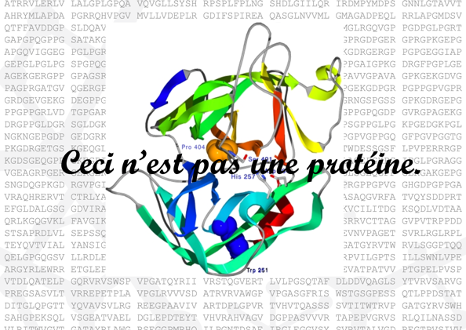
\includegraphics{./pics/magritte.png}}

}

\caption{Ceci n'est pas une proteine. Source:
https://swissmodel.expasy.org/static/course/files/PartIII\_quality\_assesment.pdf}

\end{figure}

The surrealist Belgian painter René Magritte created a collection of
surrealistic paintings entitled
\href{https://en.wikipedia.org/wiki/The_Treachery_of_Images}{\textbf{\emph{La
trahison des images}} (1928--1929)}. The most renowned of those
paintings show a smoking pipe and the following caption underneath:
``Ceci n'est pas une pipe'' (This is not a pipe). Indeed! It is the
painting of a pipe.

Similarly, a picture of a protein, or a PDF file with the coordinates of
a protein structure, is not a protein. It is a representation of ONE
structure. Even experimentally determined structures have important
limitations that we should always keep in mind: (1) they are a fixed
structure whereas proteins \emph{in vivo} are flexible and dynamic and
(2) they are subjected to experimental error and they often contain
regions of low reliability. That does not mean that protein structures
are useless, they can be very useful, but we must be aware of the
limitations as well as the applications.

\hypertarget{before-going-forward-protein-structure-101}{%
\chapter{Before going forward: Protein Structure
101}\label{before-going-forward-protein-structure-101}}

Although you can make some protein modeling without being an expert in
structural biology, a basic understanding of protein structure is
strongly advisable. Over the years, I noticed that graduate students in
biology, biomedicine and related fields have very different background
on protein structure. If you want to review and update your background
on protein structure, I recommend you the great review by Stollar and
Smith (2020) and the wikipedia articles on protein structures
(\url{https://en.wikipedia.org/wiki/Protein_structure}), which
constituted my main source for this section.

\begin{figure}

{\centering 

\href{https://en.wikipedia.org/wiki/Protein_structure}{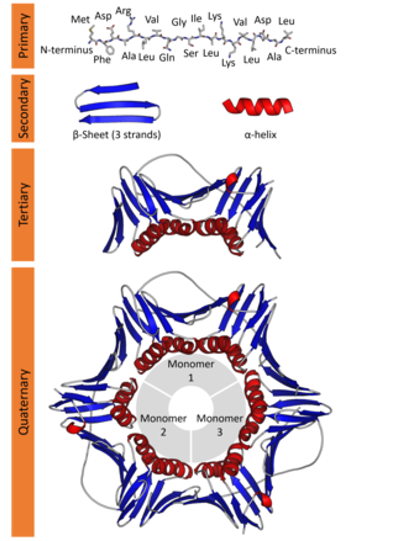
\includegraphics{./pics/Protein_structure.png}}

}

\caption{Protein structure levels, using human PCNA (PDB 1AXC) as an
example.}

\end{figure}

Proteins are key components of life, playing key roles in almost any
possible vital function, either as passive, scaffolding elements or as
active enzymes that catalyze metabolic reactions. Proteins are built as
polymers of amino acids and the sequence of amino acids of a particular
protein can be also called \textbf{the primary structure} of the
protein. Amino acids chains can spontaneously fold up into
three-dimensional structures, mostly stabilized by hydrogen bonds
between amino acids.~ The amino acid sequence determine different layers
of 3D structure. Each of the 20 natural amino acids has different
physicochemical properties that affect its preferred conformation. Thus,
a first level of folding is called \textbf{secondary structure}, forming
common patterns as we will see in a moment.

\begin{figure}

{\centering 

\href{https://www.reddit.com/r/chemistry/comments/acyald/venn_diagram_showing_the_properties_of_the_20/}{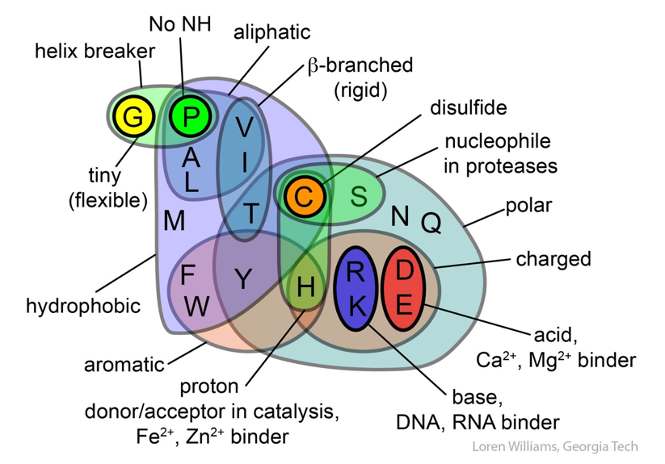
\includegraphics{./pics/aa.png}}

}

\caption{Amino acids clasification by type}

\end{figure}

These stretches of secondary structure patterns can fold in 3D due to
interactions between the side chains of amino acids. This is called
protein tertiary structure. Finally, two or more individual peptides
chains can form a~ multisubunit proteins that have the so-called
\textbf{quaternary structure}.

It should be noted that the peptide bond itself cannot rotate as it has
double bond-like character. Therefore, rotation can only occur about the
bond between the Cα and the C = O group, (the phi (φ) angle) and the Cα
and the NH group, (the psi (ψ) angle). In effect, the polypeptide
backbone chain is composed of a repeating series of two rotatable bonds
followed by one non-rotatable (peptide) bond. However, not all 360º of
the psi and phi angles are possible as neighbouring sidechains can clash
due to steric hindrance. In effect, for certain angles and amino acid
combinations, the atoms cannot be in the same physical place and this
partly explains why some amino acids have a higher propensity
(likelihood) to form different types of secondary structure.

\begin{figure}

{\centering 

\href{https://portlandpress.com/essaysbiochem/article/64/4/649/226515/Uncovering-protein-structure}{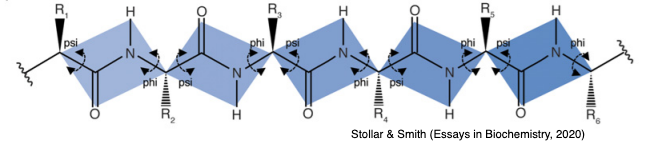
\includegraphics{./pics/peptide_bond.png}}

}

\caption{Scheme of a generic polypeptide chain. Residue side chains are
denoted as R. Coloured rectangles indicate sets of six atoms that are
coplanar due to the double-bond character of the peptide bond. Arrows
indicate the bonds that are free to rotate with the angle of rotation
about the N--Cα known as phi and about the Cα--C known as psi. Note that
only peptide backbone bonds are labelled, in most cases the R group bond
is free to rotate.}

\end{figure}

Within these restraints, the two principal local conformations that
avoid steric hindrance and maximise backbone--backbone hydrogen bonding
are the α-helix and the β-sheet secondary structures. The α-helix is a
right-handed coil in which backbone NH group hydrogen bonds to the
backbone C = O group of the amino acid located four residues earlier
along the protein sequence. This results in a polypeptide chain that
twists in a regular coil shape with the R-groups pointing outwards away
from the peptide backbone. It takes approximately 3.6 residues to
complete a full turn of a helix.

\begin{figure}

\begin{minipage}[t]{0.50\linewidth}

{\centering 

\raisebox{-\height}{

\href{https://en.wikipedia.org/wiki/Alpha_helix}{\includegraphics{./pics/alpha.gif}}

}

\caption{Alpha helix}

}

\end{minipage}%
%
\begin{minipage}[t]{0.50\linewidth}

{\centering 

\raisebox{-\height}{

\href{https://en.wikipedia.org/wiki/Beta_sheet}{\includegraphics{./pics/Animated_Beta_sheet.gif}}

}

\caption{Beta sheet}

}

\end{minipage}%

\end{figure}

Different amino-acid sequences have different propensities for forming
α-helical structure.
\href{https://en.wikipedia.org/wiki/Methionine}{Methionine},
\href{https://en.wikipedia.org/wiki/Alanine}{alanine},
\href{https://en.wikipedia.org/wiki/Leucine}{leucine},
\href{https://en.wikipedia.org/wiki/Glutamate}{glutamate}, and
\href{https://en.wikipedia.org/wiki/Lysine}{lysine} have especially high
helix-forming propensities, whereas
\href{https://en.wikipedia.org/wiki/Proline}{proline} and
\href{https://en.wikipedia.org/wiki/Glycine}{glycine} have poor
helix-forming propensities.
\href{https://en.wikipedia.org/wiki/Proline}{Proline} either breaks or
kinks a helix, both because it cannot donate an amide
\href{https://en.wikipedia.org/wiki/Hydrogen_bond}{hydrogen bond}
(having no amide hydrogen), and also because its bulky sidechain
interferes sterically with the backbone of the preceding turn. However,
proline is often seen as the \emph{first} residue of a helix, it is
presumed due to its structural rigidity. At the other extreme,
\href{https://en.wikipedia.org/wiki/Glycine}{glycine} also tends to
disrupt helices because its high conformational flexibility makes it
entropically expensive to adopt the relatively constrained α-helical
structure.

β-sheets are composed of two or more extended polypeptide chains called
β-strands that run alongside each other. They can be arranged in either
a parallel or antiparallel manner. The residues arrange themselves in a
regular zigzag manner with the adjacent peptide bonds pointing in
opposite directions. In this arrangement, the NH group and the C = O
group of each amino acid is hydrogen-bonded to the C = O group and NH
group respectively on the adjacent strands. Chains can run in opposite
directions, forming an antiparallel β-sheet, or in the same direction,
forming a parallel β-sheet. Sidechains from each of the residues point
away from the sheets and alternate in opposite directions between
residues. It is common to see a pattern of alternating hydrophilic and
hydrophobic residues in the primary structure, giving the β-sheets
hydrophilic and hydrophobic faces.

Large aromatic residues
(\href{https://en.wikipedia.org/wiki/Tyrosine}{tyrosine},
\href{https://en.wikipedia.org/wiki/Phenylalanine}{phenylalanine},
\href{https://en.wikipedia.org/wiki/Tryptophan}{tryptophan}) and
β-branched amino acids
(\href{https://en.wikipedia.org/wiki/Threonine}{threonine},
\href{https://en.wikipedia.org/wiki/Valine}{valine},
\href{https://en.wikipedia.org/wiki/Isoleucine}{isoleucine}) are favored
to be found in β-strands. As i the case of α-helixes, β-strands are
often ended by \href{https://en.wikipedia.org/wiki/Glycine}{glycines},
which are especially common in β-turns (the most common conector between
strands), as \href{https://en.wikipedia.org/wiki/Amino_acid}{amino
acids} with positive φ angles.

\hypertarget{playing-with-secondary-structures}{%
\subsection{Playing with secondary
structures}\label{playing-with-secondary-structures}}

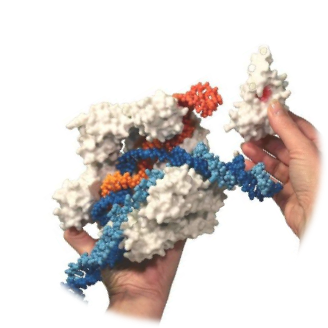
\includegraphics{./pics/handson.png}

There are a few online alternatives to model any peptide sequence and
quickly see the effect of amino acids composition in the secondary
structure. One of the best-known is Foldit
(\href{http://www.fold.it}{www.fold.it}, Miller et al. (2020)), a gaming
platform for biochemistry and structural biology teaching. It is a
highly recommended alternative for most courses related with protein
structure.

In this course we are going to try a more recent proposal, recently
twitted by Sergey Ovchinnikov (see
\url{https://twitter.com/sokrypton/status/1535857255647690753}). It is
based on ColabFold (see \url{https://github.com/sokrypton/ColabFold}~
and Mirdita et al. (2022)), an Alphafold2 (see Jumper et al. (2021))
free notebook in \href{https://colab.research.google.com/?hl=en}{Google
Colab notebook}. All you need is a Google account a the following
``cheatsheet''.

\begin{figure}

{\centering 

\href{https://twitter.com/sokrypton/status/1535857255647690753}{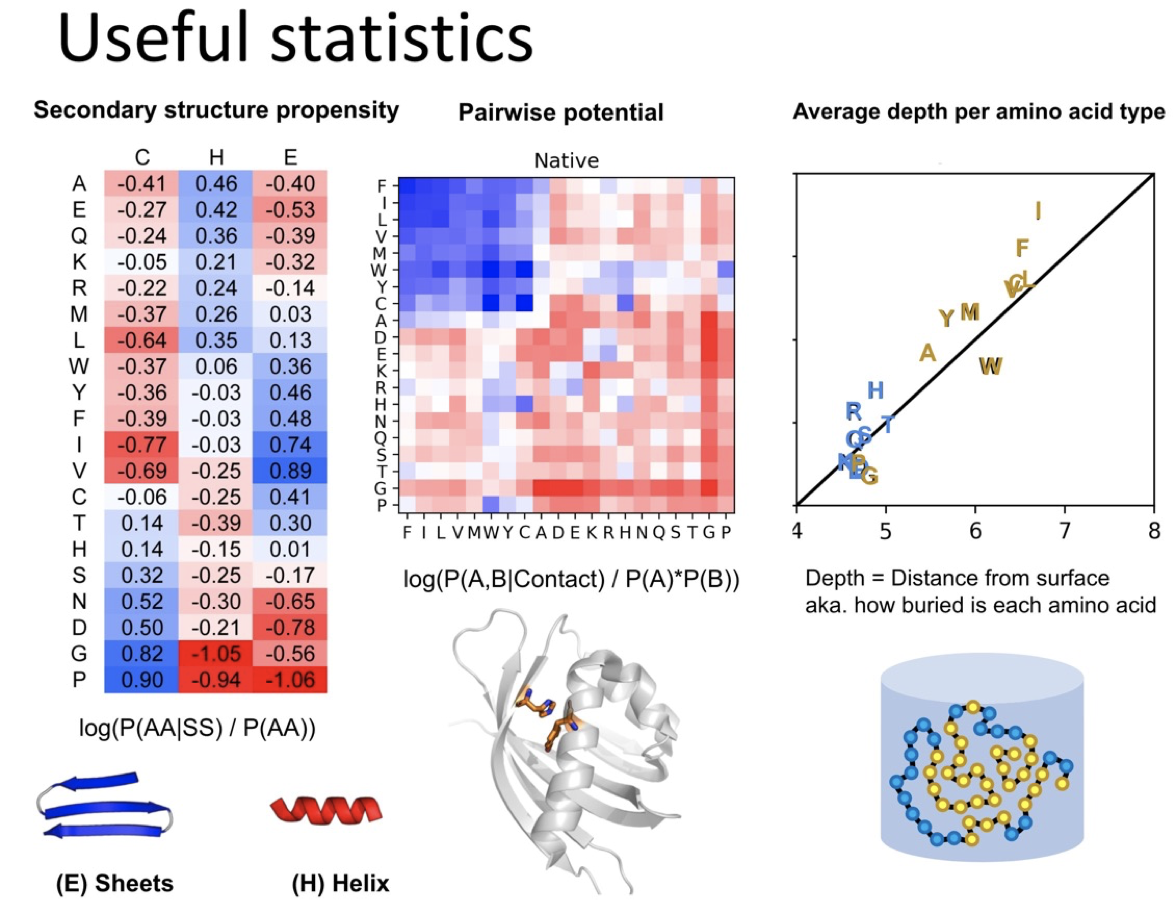
\includegraphics{./pics/cheatsheet.png}}

}

\caption{Basic protein amino acids stats for protein design with
ColabFold Single}

\end{figure}

Now go to ColabFold Single:
\url{https://colab.research.google.com/github/sokrypton/af_backprop/blob/beta/examples/AlphaFold_single.ipynb}

Construct some small proteins and compare the output. Note that the
first model will take 3-5 min, but the others will be fasters. I provide
here some interesting examples (one-letter amino acid code):

\begin{enumerate}
\def\labelenumi{\arabic{enumi}.}
\item
  GGGGGGGGGGGGGGGGGGGGGGGGGGGGGGGGGGGGGGGG
\item
  AAAAAAAAAAAAAAAAAAAAAAAAAAAAAAAAAAAAAAAAAAAAAA
\item
  VVVVVVVVVVVVVVVVVVVVVVVVVVVVVVVVVVVVVVVVVVVVVVV
\item
  PVAVEARENGRLAVRVEGAIAVLIRENGRLVVRVEGG
\item
  ACTWEGNKLTCA
\item
  MPELEKHREELGEFLKKENTELEKHREELJEFLKKENLTELEKHREELJEFLKKENQ
\item
  GIAVEIRENGRLEVRVEGGIAVEIRENGRLEVRVEGGIAVEIRENGRLEVRVEG
\item
  MPELEKHREELGEFLKKENGIAVEIRENGRLEVRVEGYTDVKIEGGTERLKRFLEELR
\item
  Creative challenge:

  \begin{itemize}
  \item
    Two helixes
  \item
    4 strands beta-sheet
  \item
    Alpha-beta-beta-alpha
  \end{itemize}
\end{enumerate}

\hfill\break

\begin{center}\rule{0.5\linewidth}{0.5pt}\end{center}

\hypertarget{references}{%
\chapter{References}\label{references}}

\hypertarget{homology-modeling}{%
\chapter{Homology Modeling}\label{homology-modeling}}

\hypertarget{homology-modeling-1}{%
\chapter{Homology Modeling}\label{homology-modeling-1}}

\hypertarget{references-1}{%
\chapter*{References}\label{references-1}}
\addcontentsline{toc}{chapter}{References}

\hypertarget{refs}{}
\begin{CSLReferences}{1}{0}
\leavevmode\vadjust pre{\hypertarget{ref-callaway2020}{}}%
Callaway, Ewen. 2020. {``Revolutionary Cryo-EM Is Taking over Structural
Biology.''} \emph{Nature} 578 (7794): 201--1.
\url{https://doi.org/10.1038/d41586-020-00341-9}.

\leavevmode\vadjust pre{\hypertarget{ref-jumper2021}{}}%
Jumper, John, Richard Evans, Alexander Pritzel, Tim Green, Michael
Figurnov, Olaf Ronneberger, Kathryn Tunyasuvunakool, et al. 2021.
{``Highly Accurate Protein Structure Prediction with AlphaFold.''}
\emph{Nature} 596 (7873): 583--89.
\url{https://doi.org/10.1038/s41586-021-03819-2}.

\leavevmode\vadjust pre{\hypertarget{ref-miller2020}{}}%
Miller, Josh Aaron, Firas Khatib, Haley Hammond, Seth Cooper, and Scott
Horowitz. 2020. {``Introducing Foldit Education Mode.''} \emph{Nature
Structural \& Molecular Biology} 27 (9): 769--70.
\url{https://doi.org/10.1038/s41594-020-0485-6}.

\leavevmode\vadjust pre{\hypertarget{ref-mirdita2022}{}}%
Mirdita, Milot, Konstantin Schütze, Yoshitaka Moriwaki, Lim Heo, Sergey
Ovchinnikov, and Martin Steinegger. 2022. {``ColabFold: making protein
folding accessible to all.''} \emph{Nature Methods} 19 (6): 679--82.
\url{https://doi.org/10.1038/s41592-022-01488-1}.

\leavevmode\vadjust pre{\hypertarget{ref-stollar2020}{}}%
Stollar, Elliott J, and David P Smith. 2020. {``Uncovering Protein
Structure.''} \emph{Essays in Biochemistry} 64 (4): 649--80.
\url{https://doi.org/10.1042/EBC20190042}.

\end{CSLReferences}



\end{document}
